\newpage
	\section{Цель и задачи работы}
		\textbf{Цель работы}: Дополнить грамматику блоком, состоящим из последовательности операторов присваивания. 
			Для реализации предлагаются два варианта расширенной грамматики.


%%%%%%%%%%%%%%%%%%%%%%%%%%%%%%
	\section{Листинг}
        
        \lstset{inputencoding=utf8x, extendedchars=\true, breaklines=true, numbers=left,
        keywordstyle=\color{blue}, commentstyle=\color{red}}
        
        \subsection{main.py}
        \lstinputlisting[language=python]{../../main.py}

        \subsection{ll.py}
        \lstinputlisting[language=python]{../../ll.py}


%%%%%%%%%%%%%%%%%%%%%%%%%%%%%%

	\section{Тесты}
		\subsection{$\{x=2==2\}$}
			\begin{figure}[h]
				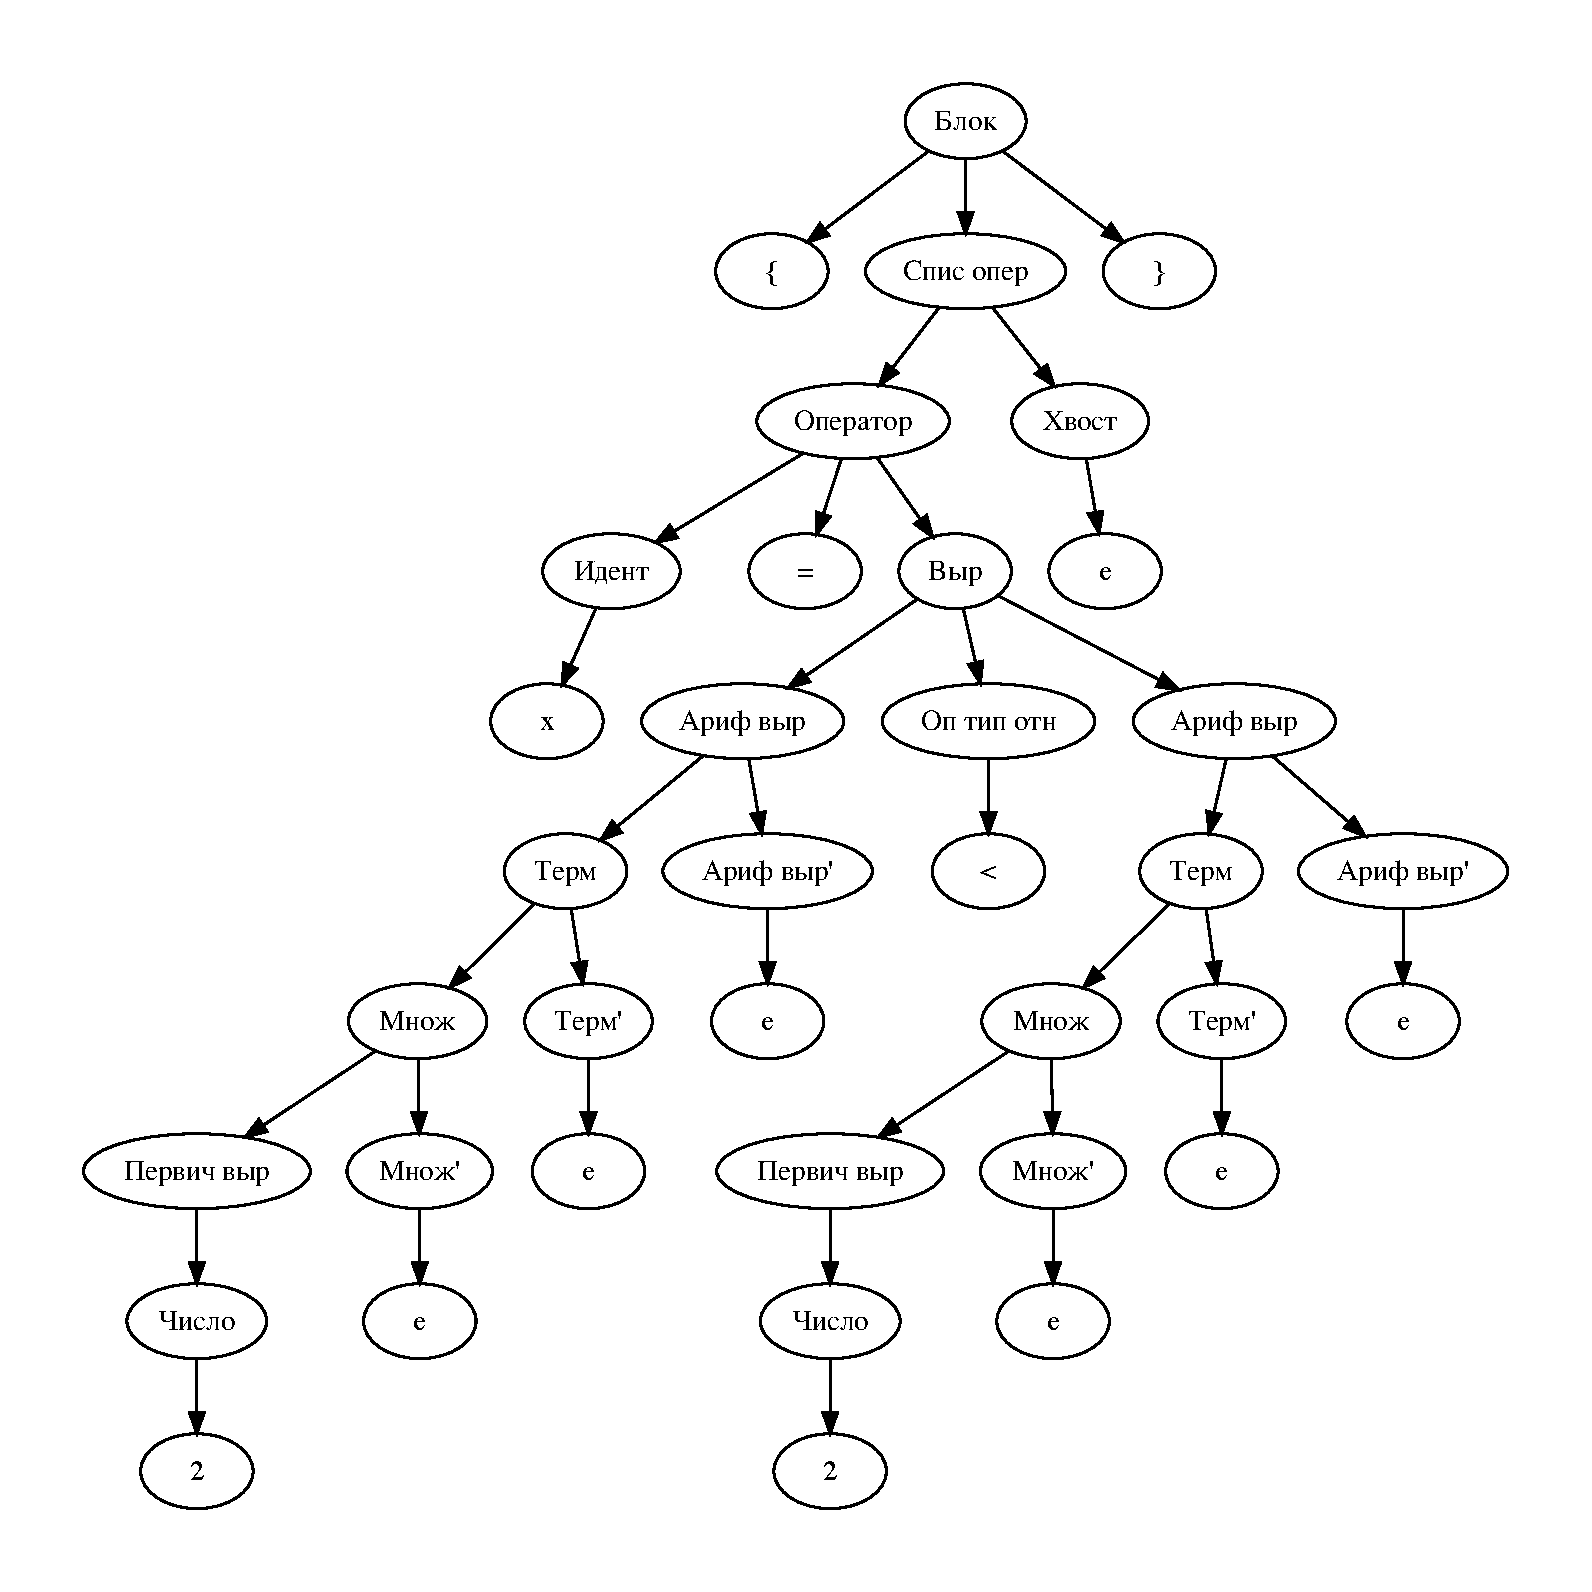
\includegraphics[scale=0.7]{2l2.png}
			\end{figure}

		\newpage

		\subsection{$\{x=2*3>=2/4\}$}
			\begin{figure}[h]
				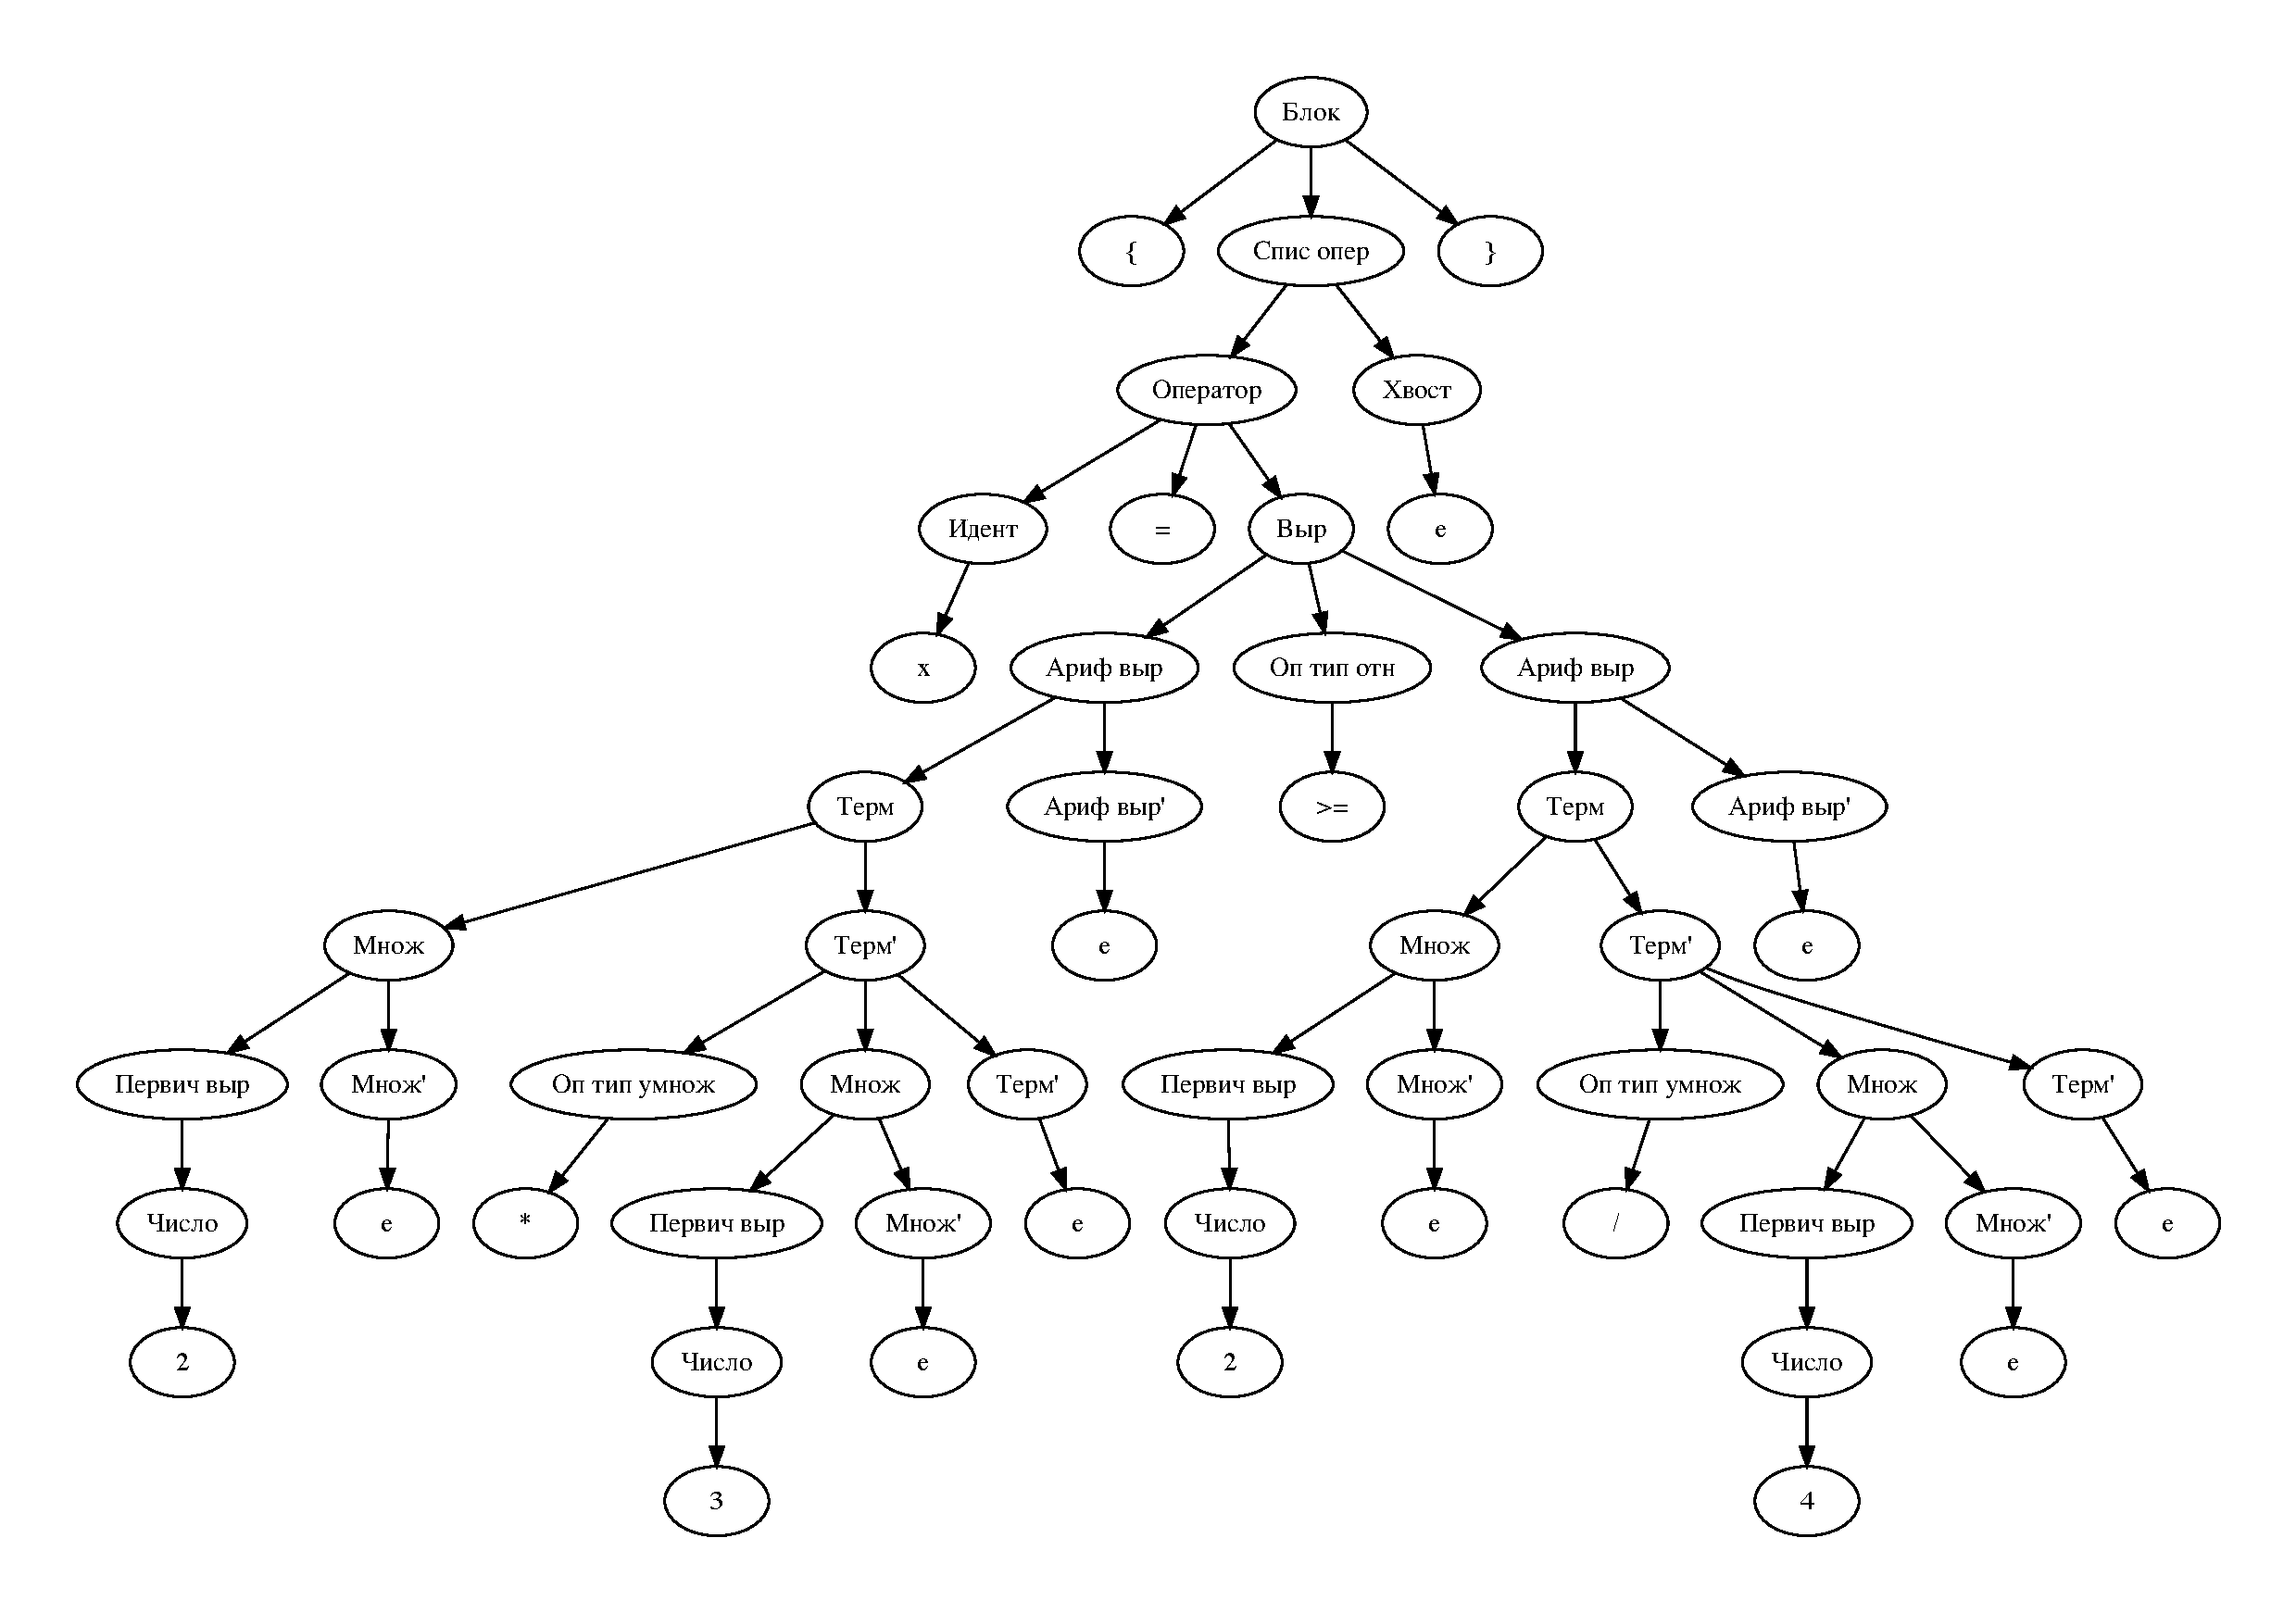
\includegraphics[scale=0.45]{2m3ge2d4.png}
			\end{figure}

		\newpage

		\subsection{$\{x=(2+3)<2\}$}
			\begin{figure}[h]
				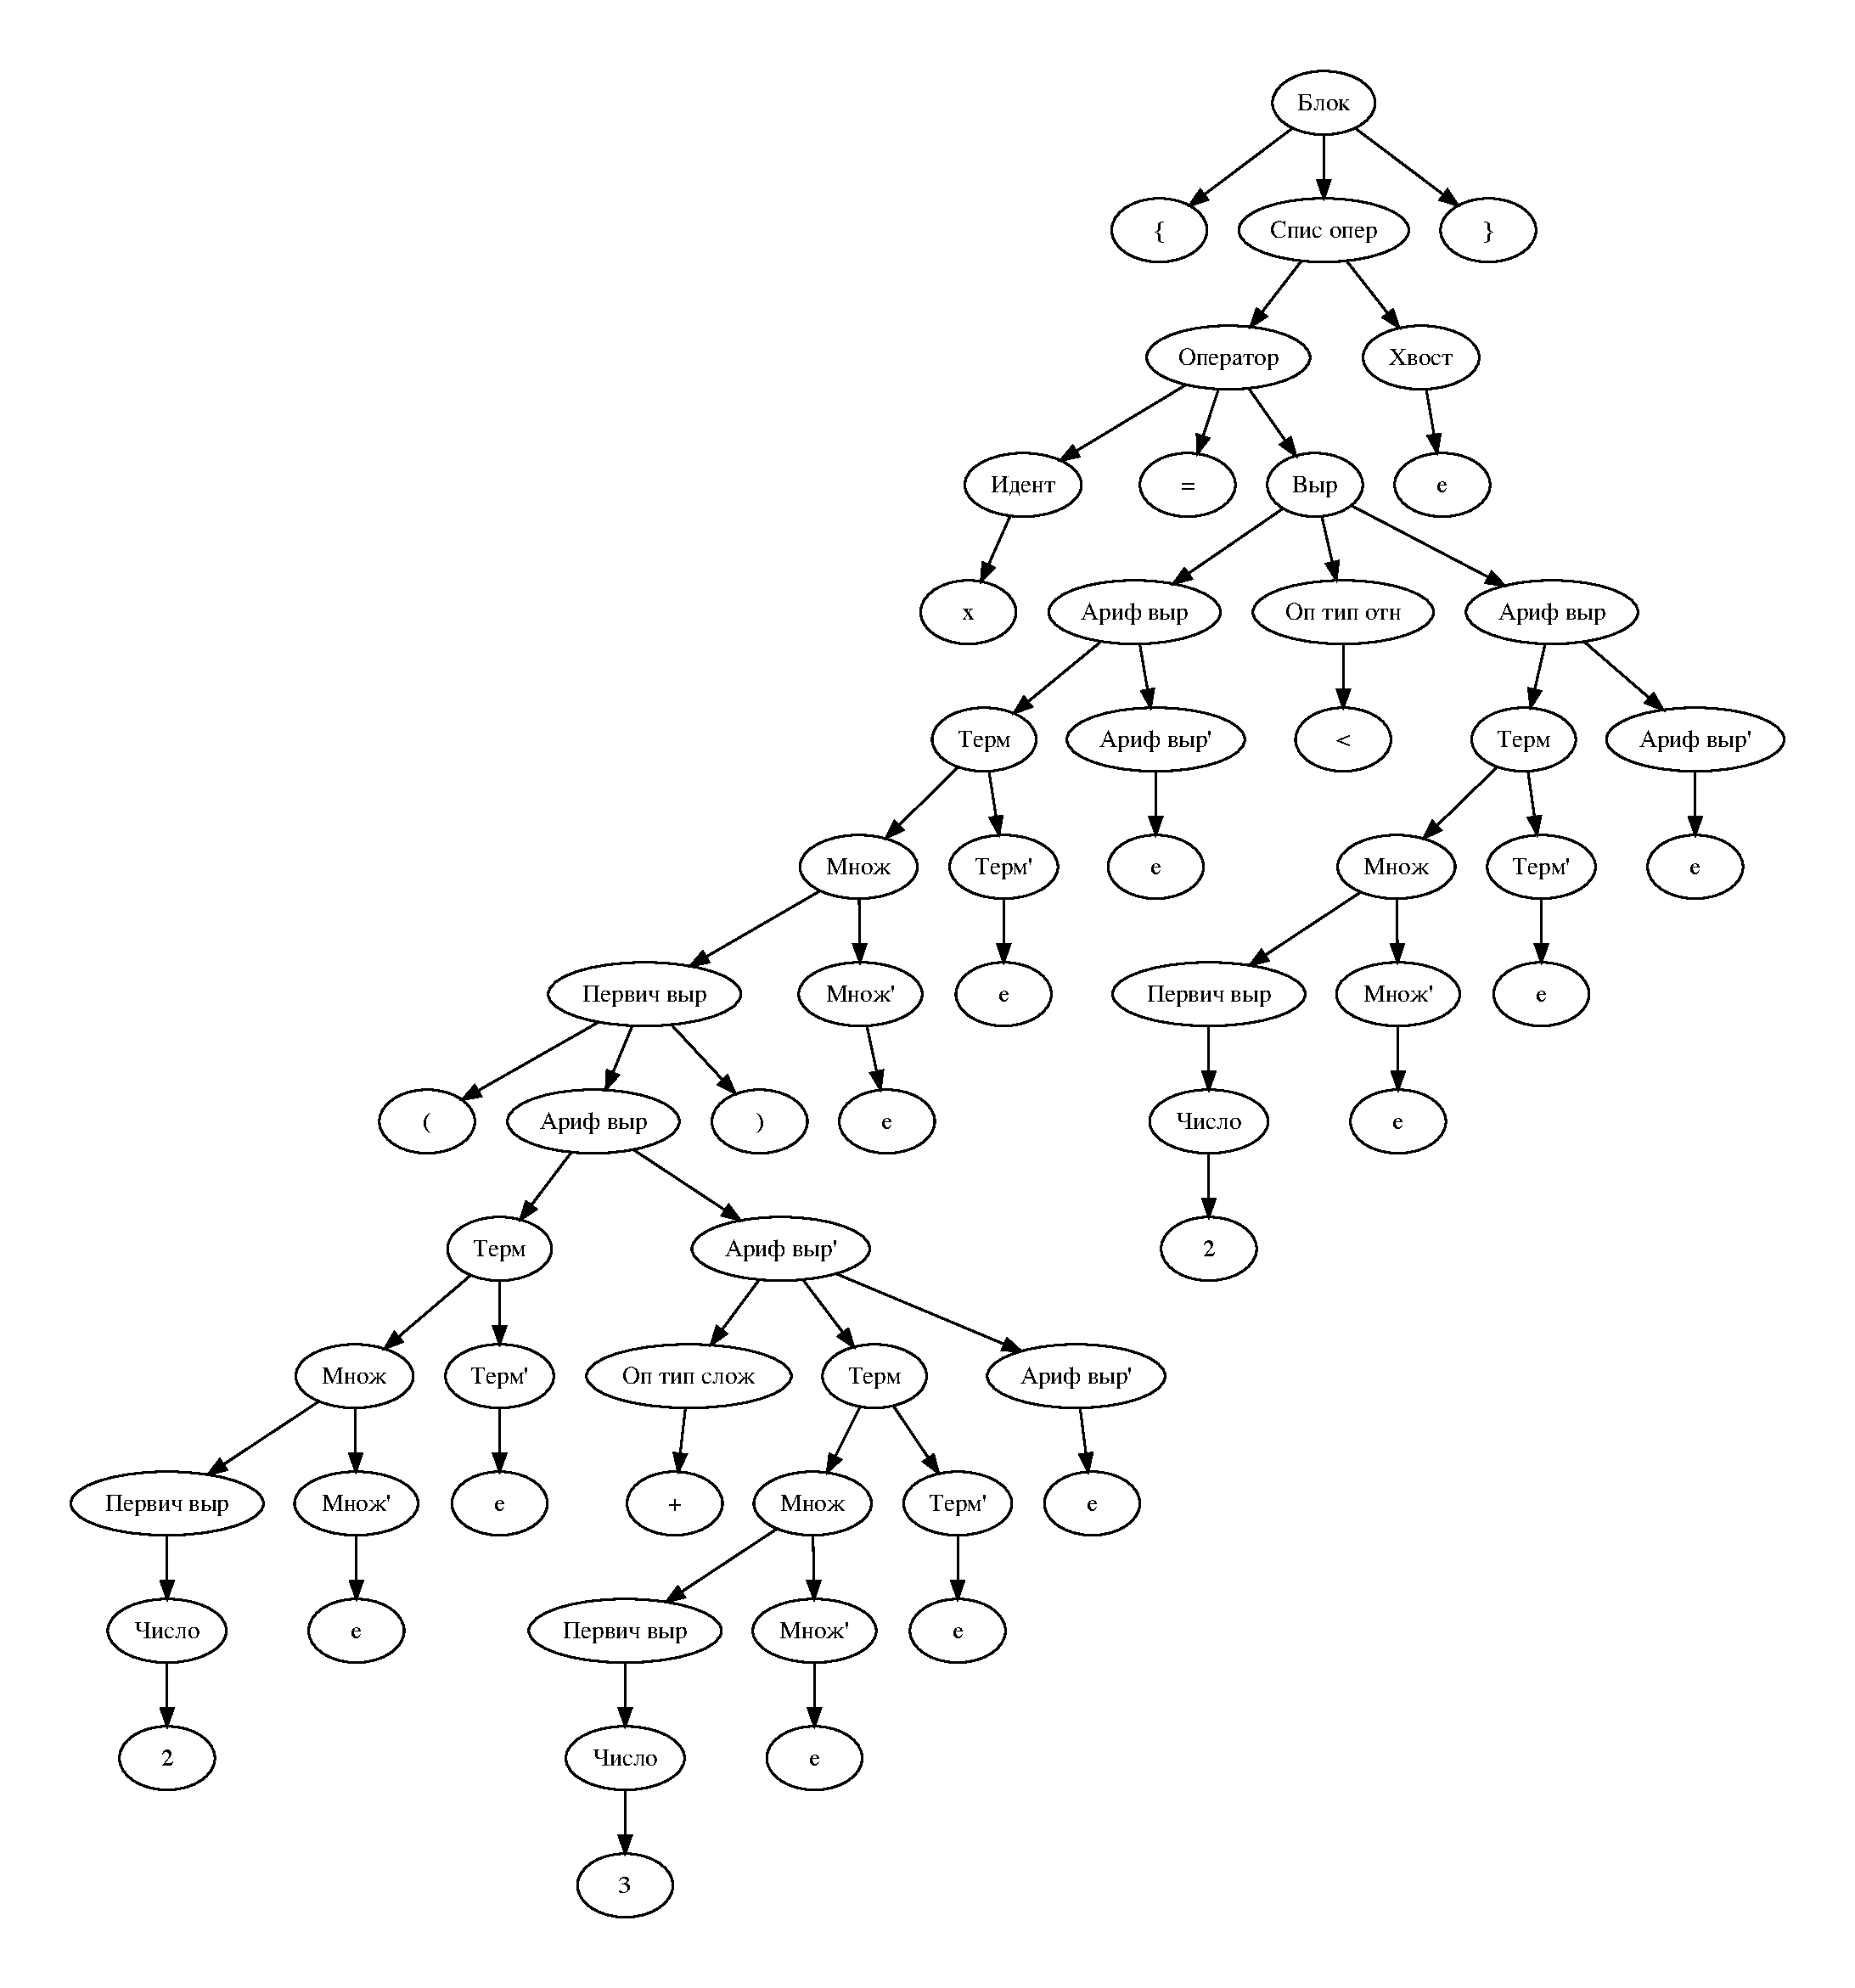
\includegraphics[scale=0.5]{p2p3pl2.png}
			\end{figure}

		\subsection{$\{x=2===2\}$}
			Дерево не построится -- ошибка входной строки

		\subsection{$\{x=2=3/4==2\}$}
			Дерево не построится -- ошибка входной строки


%%%%%%%%%%%%%%%%%%%%%%%%%%%%%%

	\newpage
	\section{Выводы}
	
	По результатам проведенной работы студент приобрел практические навыки в реализации алгоритма синтаксического разбора 
		с использованием рекурсивного спуска

%%%%%%%%%%%%%%%%%%%%%%%%%%%%%%

	\section{Список литературы}
		\begin{enumerate}
			\item БЕЛОУСОВ А.И., ТКАЧЕВ С.Б. Дискретная математика: Учеб. Для вузов / Под ред. В.С. Зарубина, А.П. Крищенко. – М.: Изд-во МГТУ им. Н.Э. Баумана, 2001.
			\item АХО А., УЛЬМАН Дж. Теория синтаксического анализа, перевода и компиляции: В 2-х томах. Т.1.: Синтаксичечкий анализ. - М.: Мир, 1978.
			\item АХО А.В, ЛАМ М.С., СЕТИ Р., УЛЬМАН Дж.Д. Компиляторы: принципы, технологии и инструменты. – М.: Вильямс, 2008.
		\end{enumerate}
	